\chapter{Oxidação e redução dos alcenos}\label{ch:b2:alkene-redox}

A cola epóxi de dois componentes vem em dois tubos: um contém moléculas
terminadas em anéis \omterm{def:b2:alkene-redox:epoxide}{epóxido}, anéis de três membros com dois carbonos e um
oxigênio; o outro, uma amina. Misturados, os anéis tensionados se abrem um
após o outro e a pasta endurece em uma rede rígida. Os alcenos são a
matéria-prima desses anéis, de álcoois colocados onde a regra de Markovnikov
nunca os poria, de dióis com uma geometria escolhida e dos pequenos fragmentos
que antes indicavam aos químicos onde ficava uma ligação dupla em uma
molécula. Este capítulo acrescenta às adições eletrofílicas do volume do 1.º
ano as reações que reduzem ou oxidam a ligação dupla, e a estereoquímica que
cada uma impõe.

\begin{recall}
O volume do 1.º ano: adições eletrofílicas, regra de Markovnikov, íons
halônio, adições syn e anti, hidratação dos alcenos, níveis de oxidação do
carbono, doadores de hidreto, quimiosseletividade, compostos meso e misturas
racêmicas, reações estereoespecíficas. \Cref{ch:b2:catalytic-cycles}: o ciclo
de hidrogenação do catalisador de Wilkinson.
\end{recall}

\begin{omfigure}
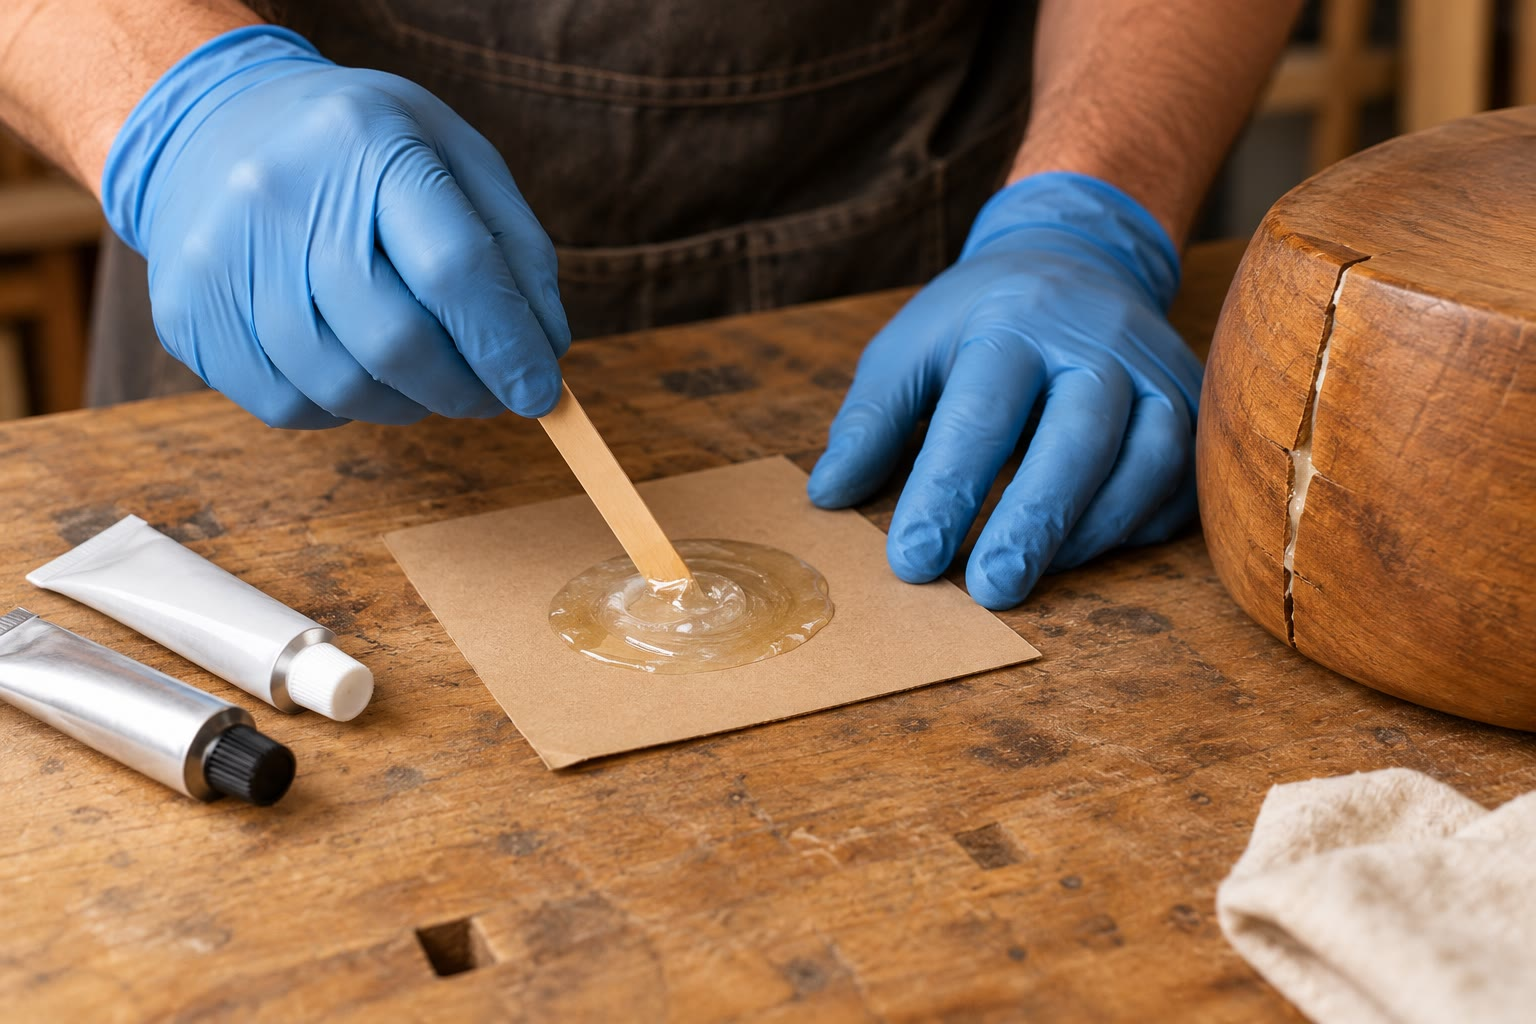
\includegraphics[width=0.6\linewidth]{images/book3/ai/b2-21-epoxy.jpg}

{\small A mistura de uma cola epóxi de dois componentes: a resina, com grupos
\omterm{def:b2:alkene-redox:epoxide}{epóxido}, e o endurecedor, uma amina, reagem assim que se encontram; os anéis
se abrem e ligam as moléculas em uma rede sólida.}
\end{omfigure}

\section{Hidrogenação catalítica}

\begin{definition}[Hidrogenação catalítica]\label{def:b2:alkene-redox:hydrogenation}
Uma \emph{hidrogenação catalítica}\index{hidrogenacao catalitica@hidrogenação catalítica} adiciona
di-hidrogênio a uma ligação múltipla na presença de um catalisador: um metal
finamente dividido (paládio sobre carvão, platina, níquel) em catálise
heterogênea, ou um complexo solúvel, como o de Wilkinson, em catálise
homogênea.
\end{definition}

Sobre uma superfície metálica, o di-hidrogênio e o alceno são ambos retidos, a
ligação \ce{H-H} é rompida em átomos de hidrogênio de superfície, e estes são
transferidos um após o outro aos átomos de carbono do alceno, que fica deitado
sobre o metal.

\begin{proposition}[Adição syn]\label{prop:b2:alkene-redox:syn-hydrogenation}
A \omterm{def:b2:alkene-redox:hydrogenation}{hidrogenação catalítica} leva os dois átomos de hidrogênio à mesma face da
ligação dupla. Um alcino hidrogenado sobre um catalisador de paládio
envenenado para no alceno, que é o isômero (\textit{Z}).
\end{proposition}

\begin{proof}[Raciocínio]
O alceno está ligado ao catalisador por uma face, e os dois hidrogênios vêm do
catalisador, por essa face: adição syn. Com um alcino, os dois hidrogênios
adicionados à ligação tripla ficam do mesmo lado, cis um em relação ao outro:
o (\textit{Z})-alceno. Um catalisador parcialmente desativado (paládio sobre
carbonato de cálcio com um sal de chumbo e quinolina) liga o alcino muito
mais fortemente que o alceno formado, que deixa a superfície antes de uma
segunda adição.
\end{proof}

\section{Hidroboração--oxidação}

\begin{definition}[Hidroboração]\label{def:b2:alkene-redox:hydroboration}
Uma \emph{hidroboração}\index{hidroboracao@hidroboração} adiciona uma ligação B--H de um borano a
uma ligação \ce{C=C}; seguida de oxidação por peróxido de hidrogênio alcalino,
ela converte o alceno em um álcool cujo grupo hidroxila fica no carbono menos
substituído: uma \emph{orientação anti-Markovnikov}\index{orientacao anti-Markovnikov@orientação anti-Markovnikov}.
\end{definition}

\begin{omfigure}
\setchemfig{atom sep=1.8em}
\schemestart[][west]
\chemfig{H_3C-[:30]CH=[:-30]CH_2}
\+ \chemfig{H-BH_2}
\arrow{->[adição syn]}
\chemfig{H_3C-[:30]CH_2-[:-30]CH_2-[:30]BH_2}
\arrow{->[\ce{H2O2}][\ce{HO-}]}
\chemfig{H_3C-[:30]CH_2-[:-30]CH_2-[:30]OH}
\schemestop
\par\vspace{6pt}

{\small Hidroboração--oxidação do propeno. O borano se adiciona em uma etapa, o
boro ao carbono terminal e o hidrogênio ao interno, ambos na mesma face; a
oxidação substitui o boro por \ce{OH} com retenção de configuração. Forma-se o
propan-1-ol, e não o propan-2-ol da hidratação catalisada por ácido.}
\end{omfigure}

\begin{proposition}[Orientação da hidroboração]\label{prop:b2:alkene-redox:hydroboration-regio}
O boro se adiciona ao carbono menos substituído da ligação dupla, e o
hidrogênio ao mais substituído; a adição é syn.
\end{proposition}

\begin{proof}[Raciocínio]
O boro, com um orbital p vazio, é o eletrófilo: no estado de transição de
quatro centros (os dois carbonos, o boro e o hidrogênio), a ligação com o boro
se forma um pouco antes da ligação C--H, e uma carga parcial positiva se
desenvolve no outro carbono, mais bem suportada pelo mais substituído; o
volumoso grupo boro também prefere a extremidade menos impedida. As duas novas
ligações se formam na mesma face, em uma etapa concertada: syn.
\end{proof}

\begin{proposition}[Oxidação com retenção]\label{prop:b2:alkene-redox:retention}
A oxidação de um alquilborano por peróxido de hidrogênio alcalino substitui
cada ligação C--B por uma ligação C--OH com retenção de configuração no carbono.
\end{proposition}

\begin{proof}[Raciocínio]
O ânion hidroperóxido se adiciona ao boro; um grupo alquila migra então do
boro para o oxigênio vizinho, com seu par de elétrons, enquanto o hidróxido
sai; o carbono mantém suas ligações do mesmo lado durante todo o processo. A
hidrólise da ligação B--O libera o álcool.
\end{proof}

\section{Os epóxidos}

\begin{definition}[Epóxido]\label{def:b2:alkene-redox:epoxide}
Um \emph{epóxido}\index{epoxido@epóxido} (oxirano) é um éter cíclico com um anel de três
membros formado por dois carbonos e um oxigênio. Uma
\emph{epoxidação}\index{epoxidacao@epoxidação} converte um alceno em um epóxido, em geral com
um \emph{perácido}\index{peracido@perácido} \ce{RCO3H}, que transfere um átomo de oxigênio à
ligação dupla.
\end{definition}

\begin{omfigure}
\setchemfig{atom sep=2em}
\schemestart
\chemfig{R-[:30]CH=[:-30]CH-[:30]R}
\+ \chemfig{Ar-C(=[2]O)-O-O-H}
\arrow{->}
\chemfig{[:-60]CH(-[:210]R)*3(-CH(-[:-30]R)-O-)}
\+ \chemfig{Ar-C(=[2]O)-OH}
\schemestop
\par\vspace{6pt}

{\small \omterm{def:b2:alkene-redox:epoxide}{Epoxidação} por um \omterm{def:b2:alkene-redox:epoxide}{perácido} (Ar: por exemplo, um grupo 3-clorofenila). O
oxigênio terminal do \omterm{def:b2:alkene-redox:epoxide}{perácido} é transferido à ligação dupla em uma etapa, com
as duas ligações C--O se formando na mesma face.}
\end{omfigure}

\begin{proposition}[Epoxidação estereoespecífica]\label{prop:b2:alkene-redox:epoxidation}
A \omterm{def:b2:alkene-redox:epoxide}{epoxidação} por um \omterm{def:b2:alkene-redox:epoxide}{perácido} é estereoespecífica: um (\textit{Z})-alceno dá o
\omterm{def:b2:alkene-redox:epoxide}{epóxido} cis, e um (\textit{E})-alceno, o \omterm{def:b2:alkene-redox:epoxide}{epóxido} trans.
\end{proposition}

\begin{proof}
O oxigênio é transferido em uma etapa concertada a uma face da ligação dupla,
que não gira nesse meio-tempo: as posições relativas dos substituintes são
conservadas.
\end{proof}

\begin{proposition}[Abertura dos epóxidos]\label{prop:b2:alkene-redox:opening}
Um nucleófilo abre um \omterm{def:b2:alkene-redox:epoxide}{epóxido} atacando um carbono pela face oposta ao
oxigênio (abertura anti, com inversão nesse carbono). Em meio básico, ele
ataca o carbono menos impedido; em meio ácido, o mais substituído.
\end{proposition}

\begin{proof}[Raciocínio]
A tensão do anel torna fáceis de romper as ligações C--O. Com um nucleófilo
forte e sem ácido, a abertura é uma substituição bimolecular, e o carbono
menos impedido é o mais facilmente alcançado. Em meio ácido, o oxigênio é
protonado; a ligação C--O com o carbono mais substituído é a que mais se
alonga, pois esse carbono tem a maior carga parcial positiva, e mesmo um
nucleófilo fraco (a água, um álcool) ataca ali --- ainda por trás, portanto
ainda anti.
\end{proof}

\begin{omfigure}
\setchemfig{atom sep=2em}
\schemestart
\chemfig{[:-60]C(-[:210]H_3C)(-[:150]H_3C)*3(-CH_2-O-)}
\arrow{->[\ce{CH3O-}][\ce{CH3OH}]}[,1.4]
\chemfig{H_3C-C(-[2]CH_3)(-[6]OH)-CH_2-OCH_3}
\schemestop

\medskip
\schemestart
\chemfig{[:-60]C(-[:210]H_3C)(-[:150]H_3C)*3(-CH_2-O-)}
\arrow{->[\ce{CH3OH}][\ce{H+}]}[,1.4]
\chemfig{H_3C-C(-[2]CH_3)(-[6]OCH_3)-CH_2-OH}
\schemestop
\par\vspace{6pt}

{\small Abertura do 2,2-dimetiloxirano pelo metanol. Em cima, com metóxido:
ataque no \ce{CH2}, o carbono menos impedido. Embaixo, em meio ácido: ataque no
carbono mais substituído, que suporta a maior parte da carga positiva do
\omterm{def:b2:alkene-redox:epoxide}{epóxido} protonado.}
\end{omfigure}

\section{Di-hidroxilação}

\begin{definition}[Di-hidroxilação]\label{def:b2:alkene-redox:dihydroxylation}
Uma \emph{di-hidroxilação}\index{di-hidroxilacao@di-hidroxilação} converte um alceno em um
1,2-diol adicionando um grupo \ce{OH} a cada carbono da ligação dupla.
\end{definition}

O tetróxido de ósmio, em quantidade catalítica com um reoxidante, e o
permanganato diluído a frio adicionam os dois oxigênios por meio de um éster
cíclico, em uma face: uma \omterm{def:b2:alkene-redox:dihydroxylation}{di-hidroxilação} syn. A \omterm{def:b2:alkene-redox:epoxide}{epoxidação} seguida de
abertura pela água em meio ácido dá o diol anti.

\begin{proposition}[Dióis syn e anti]\label{prop:b2:alkene-redox:diols}
A partir do (\textit{Z})-but-2-eno, a \omterm{def:b2:alkene-redox:dihydroxylation}{di-hidroxilação} syn dá o meso-butano-2,3-diol,
e a via do \omterm{def:b2:alkene-redox:epoxide}{epóxido} dá os dióis racêmicos (2\textit{R},3\textit{R}) e
(2\textit{S},3\textit{S}); a partir do (\textit{E})-but-2-eno, os resultados se
invertem.
\end{proposition}

\begin{proof}
No (\textit{Z})-but-2-eno, as duas metilas estão do mesmo lado. Adicionar dois
\ce{OH} em uma face dá um diol no qual, escrito na conformação eclipsada da
antiga ligação dupla, os dois \ce{OH} estão de um lado e as duas metilas do
outro: um plano de simetria passa entre C2 e C3, é o composto meso. A via do
\omterm{def:b2:alkene-redox:epoxide}{epóxido} coloca os dois \ce{OH} em faces opostas (anti): o plano de simetria se
perde, e o ataque em um ou outro carbono do \omterm{def:b2:alkene-redox:epoxide}{epóxido} aquiral, igualmente
provável, dá os dois enantiômeros em quantidades iguais. Para o
(\textit{E})-alceno, cada etapa muda a relação entre as metilas, o que inverte
os resultados.
\end{proof}

\begin{omfigure}
\begin{tikzpicture}[font=\small]
  \begin{scope}
    \draw[thick] (0,0) -- (0,1.2);
    \draw[thick] (0,1.2) -- (-0.7,1.45); \draw[thick] (0,1.2) -- (0.7,1.45);
    \node[anchor=east] at (-0.7,1.45) {\ce{HO}}; \node[anchor=west] at (0.7,1.45) {\ce{CH3}};
    \draw[thick] (0,0) -- (-0.7,0.25); \draw[thick] (0,0) -- (0.7,0.25);
    \node[anchor=east] at (-0.7,0.25) {\ce{HO}}; \node[anchor=west] at (0.7,0.25) {\ce{CH3}};
    \node[anchor=south] at (0,1.25) {\scriptsize H};
    \node[anchor=north] at (0,-0.05) {\scriptsize H};
    \draw[densely dashed, omThm] (-1.6,0.6) -- (1.6,0.6);
    \node at (0,-1.0) {syn: meso};
  \end{scope}
  \begin{scope}[xshift=6.5cm]
    \draw[thick] (0,0) -- (0,1.2);
    \draw[thick] (0,1.2) -- (-0.7,1.45); \draw[thick] (0,1.2) -- (0.7,1.45);
    \node[anchor=east] at (-0.7,1.45) {\ce{HO}}; \node[anchor=west] at (0.7,1.45) {\ce{CH3}};
    \draw[thick] (0,0) -- (-0.7,0.25); \draw[thick] (0,0) -- (0.7,0.25);
    \node[anchor=east] at (-0.7,0.25) {\ce{H3C}}; \node[anchor=west] at (0.7,0.25) {\ce{OH}};
    \node[anchor=south] at (0,1.25) {\scriptsize H};
    \node[anchor=north] at (0,-0.05) {\scriptsize H};
    \node[align=center] at (0,-1.1) {anti: um enantiômero\\ (formado com sua imagem especular)};
  \end{scope}
\end{tikzpicture}

{\small Os dois butano-2,3-dióis obtidos do (\textit{Z})-but-2-eno, esquemáticos
(ligação C2--C3 vertical, com os dois grupos de cada carbono desenhados à
esquerda e à direita). A adição syn coloca os dois \ce{OH} do mesmo lado: um
plano de simetria interno (tracejado), o composto meso. A adição anti os
coloca em lados opostos: um diol quiral, formado com seu enantiômero.}
\end{omfigure}

\section{Clivagem oxidativa}

\begin{definition}[Clivagem oxidativa]\label{def:b2:alkene-redox:cleavage}
Uma \emph{clivagem oxidativa}\index{clivagem oxidativa} rompe as duas ligações de uma
ligação dupla \ce{C=C} e transforma cada carbono em um grupo carbonila ou
carboxila. Em uma \emph{ozonólise}\index{ozonolise@ozonólise}, o alceno reage com o ozônio e
o ozonídeo intermediário é decomposto em uma segunda etapa, o tratamento.
\end{definition}

\begin{proposition}[Produtos da ozonólise]\label{prop:b2:alkene-redox:ozonolysis}
A \omterm{def:b2:alkene-redox:cleavage}{ozonólise} divide cada ligação \ce{C=C} em dois grupos \ce{C=O}. Com um
tratamento redutor (zinco e ácido, ou sulfeto de dimetila), um carbono que tem
um hidrogênio dá um aldeído; com um tratamento oxidante (peróxido de
hidrogênio), dá um ácido carboxílico. Um carbono que tem dois grupos carbonados
dá uma cetona nos dois casos.
\end{proposition}

\begin{proof}[Raciocínio]
O ozônio se adiciona à ligação dupla, o intermediário se rearranja e a ligação
C--C se rompe, dando um ozonídeo no qual cada antigo carbono do alceno está
ligado a dois oxigênios. O tratamento o reduz a dois compostos carbonílicos,
ou oxida ainda mais os aldeídos. As etapas intermediárias são admitidas.
\end{proof}

\begin{omfigure}
\setchemfig{atom sep=2em}
\schemestart
\chemfig{H_3C-[:30]C(-[:90]CH_3)=[:-30]CH-[:30]CH_3}
\arrow{->[1. \ce{O3}][2. \ce{Zn}, \ce{H+}]}[,1.8]
\chemfig{H_3C-C(=[2]O)-CH_3}
\+
\chemfig{H-C(=[2]O)-CH_3}
\schemestop
\par\vspace{6pt}

{\small \omterm{def:b2:alkene-redox:cleavage}{Ozonólise} do 2-metilbut-2-eno com tratamento redutor: propanona e
etanal. Unir de novo os dois carbonos carbonílicos por uma ligação dupla
reconstrói o alceno.}
\end{omfigure}

\begin{method}[Localizar uma ligação dupla]\label{met:b2:alkene-redox:locate-double-bond}
\begin{enumerate}
  \item Liste os fragmentos carbonílicos da \omterm{def:b2:alkene-redox:cleavage}{ozonólise} e conte seus carbonos;
        eles devem somar os do alceno.
  \item Cada carbono de \ce{C=O} era um carbono de ligação dupla: una os
        fragmentos substituindo dois \ce{C=O} por um \ce{C=C}.
  \item Para um anel, sai uma única molécula com dois grupos carbonila; una
        suas duas extremidades.
  \item Verifique com a fórmula e com o grau de insaturação.
\end{enumerate}
\end{method}

O permanganato concentrado a quente também cliva as ligações duplas, dando
ácidos e cetonas; o periodato de sódio cliva os 1,2-dióis em dois compostos
carbonílicos, uma via mais branda passando pelo diol.

\begin{method}[Escolher um reagente para um alceno]\label{met:b2:alkene-redox:choose-reagent}
\begin{center}
\small
\renewcommand{\arraystretch}{1.15}
\begin{tabular}{lll}
alvo & reagente & estereoquímica, orientação \\ \hline
alcano & \ce{H2}, Pd/C & syn \\
álcool de Markovnikov & \ce{H2O}, ácido & via um carbocátion \\
álcool anti-Markovnikov & \ce{BH3}, depois \ce{H2O2}, \ce{HO-} & syn \\
\omterm{def:b2:alkene-redox:epoxide}{epóxido} & \omterm{def:b2:alkene-redox:epoxide}{perácido} & estereoespecífica \\
diol syn & \ce{OsO4} (cat.) ou \ce{MnO4-} a frio & syn \\
diol anti & \omterm{def:b2:alkene-redox:epoxide}{perácido}, depois \ce{H2O}, ácido & anti \\
duas carbonilas & \ce{O3}, depois \ce{Zn}/ácido & clivagem \\
\end{tabular}
\end{center}
\end{method}

\begin{safety}{\ghs[5mm]{GHS02}\,\ghs[5mm]{GHS03}\,\ghs[5mm]{GHS05}\,\ghs[5mm]{GHS06}}
O tetróxido de ósmio é volátil e muito tóxico (lesa os olhos); ele é usado em
quantidade catalítica, em solução, na capela. Os \omterm{def:b2:alkene-redox:epoxide}{perácidos} e o peróxido de
hidrogênio são oxidantes que podem se decompor violentamente quando aquecidos
ou concentrados; as soluções de borano são inflamáveis; o ozônio é tóxico e é
gerado na capela.
% ledger: ghs:OsO4, ghs:mCPBA, ghs:BH3-THF, ghs:O3, ghs:NaIO4
\end{safety}

\section{Exercícios}

\begin{exercise}[$\star$]\label{exo:b2:alkene-redox:1}
Dê o produto do 1-metilciclo-hexeno com: \ce{H2}/Pd; \ce{H2O}/\ce{H+};
\ce{BH3} e depois \ce{H2O2}/\ce{HO-}; um \omterm{def:b2:alkene-redox:epoxide}{perácido}; \ce{OsO4} (cat.); \ce{O3} e depois
\ce{Zn}/\ce{H+}.
\end{exercise}

\begin{exercise}[$\star$]\label{exo:b2:alkene-redox:2}
Que álcool a hidroboração--oxidação dá a partir do 2-metilpropeno? E a
hidratação catalisada por ácido?
\end{exercise}

\begin{exercise}[$\star$]\label{exo:b2:alkene-redox:3}
Desenhe o \omterm{def:b2:alkene-redox:epoxide}{epóxido} formado a partir do (\textit{E})-but-2-eno. Ele é quiral?
\end{exercise}

\begin{exercise}[$\star$]\label{exo:b2:alkene-redox:4}
Dê os produtos da \omterm{def:b2:alkene-redox:cleavage}{ozonólise} do hex-3-eno com um tratamento redutor e depois com
um tratamento oxidante.
\end{exercise}

\begin{exercise}[$\star\star$]\label{exo:b2:alkene-redox:5}
Dê os dióis formados a partir do (\textit{Z})-but-2-eno (a) com \ce{OsO4}; (b) com um
\omterm{def:b2:alkene-redox:epoxide}{perácido} e depois ácido aquoso. Qual é opticamente inativo por ser meso, e qual
por ser racêmico?
\end{exercise}

\begin{exercise}[$\star\star$]\label{exo:b2:alkene-redox:6}
O 2,2-dimetiloxirano é aberto pela água em meio ácido e pelo hidróxido. As duas
vias dão o mesmo produto? Explique.
\end{exercise}

\begin{exercise}[$\star\star$]\label{exo:b2:alkene-redox:7}
Como você prepararia o (\textit{Z})-hex-3-eno a partir do hex-3-ino?
\end{exercise}

\begin{exercise}[$\star\star$]\label{exo:b2:alkene-redox:8}
Um alceno \ce{C7H14} dá, por \omterm{def:b2:alkene-redox:cleavage}{ozonólise} com tratamento redutor, propanona e
butanal. Dê sua estrutura.
\end{exercise}

\begin{exercise}[$\star\star$]\label{exo:b2:alkene-redox:9}
Proponha uma síntese do hexan-1-ol a partir do hex-1-eno e diga por que a
hidratação catalisada por ácido falharia.
\end{exercise}

\begin{exercise}[$\star\star\star$]\label{exo:b2:alkene-redox:10}
O limoneno tem uma ligação dupla trissubstituída no anel e uma dissubstituída
exocíclica (\ce{C(CH3)=CH2}). Qual reage primeiro com um equivalente de
\omterm{def:b2:alkene-redox:epoxide}{perácido}, e qual com um equivalente de um borano volumoso? Explique.
\end{exercise}

\begin{exercise}[$\star\star\star$]\label{exo:b2:alkene-redox:11}
Prepare o trans-ciclo-hexano-1,2-diol a partir do ciclo-hexeno, e o cis-ciclo-hexano-1,2-diol.
\end{exercise}

\begin{exercise}[$\star\star\star$]\label{exo:b2:alkene-redox:12}
Um composto \ce{C6H10} absorve um equivalente de \ce{H2}. Sua \omterm{def:b2:alkene-redox:cleavage}{ozonólise} com
tratamento redutor dá um único produto, o hexanodial \ce{OHC-(CH2)4-CHO}.
Identifique-o.
\end{exercise}

\section{Problema: Identificar um terpeno}

\begin{problem}[{Problema de fim de semana --- a fórmula e a insaturação do
limoneno, sua hidrogenação, os fragmentos de sua ozonólise e as reações
seletivas de suas duas ligações duplas}]
\label{pb:b2:alkene-redox:1}
O limoneno, o aroma da casca da laranja, tem a fórmula \ce{C10H16}. Ele é o
1-metil-4-(prop-1-en-2-il)ciclo-hex-1-eno: uma ligação dupla no anel que leva
uma metila, e um grupo exocíclico \ce{C(CH3)=CH2} no carbono oposto do anel. $R =
\qty{8.314}{J/(K.mol)}$; massas molares (\unit{g/mol}): C 12.011, H 1.008.
% ledger: aw:C, aw:H, const:R, ghs:limonene

\medskip
\noindent\textbf{Parte I --- Fórmula e hidrogenação.}
\begin{enumerate}
  \item Calcule a massa molar do limoneno.
  \item Calcule seu grau de insaturação.
  \item Quantos anéis e quantas ligações duplas ele tem?
  \item Escreva sua hidrogenação sobre paládio, incluindo o produto.
  \item Calcule a quantidade de di-hidrogênio absorvida por \qty{1.00}{g} de limoneno.
  \item Calcule seu volume a \qty{25}{\degreeCelsius} e \qty{1.00}{bar}.
  \item O produto é quiral?
\end{enumerate}

\medskip
\noindent\textbf{Parte II --- A \omterm{def:b2:alkene-redox:cleavage}{ozonólise}.}
\begin{enumerate}[resume]
  \item Que fragmentos a \omterm{def:b2:alkene-redox:cleavage}{ozonólise} com tratamento redutor dá? (Conte os carbonos.)
  \item Por que a ligação dupla do anel dá uma molécula, e não duas?
  \item Que fragmento se perde como gás ou líquido volátil?
  \item Como os produtos difeririam com um tratamento oxidante?
  \item Mostre como os fragmentos localizam as duas ligações duplas.
  \item Quantos estereocentros tem o limoneno, e a \omterm{def:b2:alkene-redox:cleavage}{ozonólise} o conserva?
\end{enumerate}

\medskip
\noindent\textbf{Parte III --- A \omterm{def:b2:alkene-redox:hydroboration}{hidroboração}.}
\begin{enumerate}[resume]
  \item Com um equivalente de um borano volumoso, qual ligação dupla reage? Por quê?
  \item Desenhe o produto após a oxidação.
  \item O novo álcool é primário, secundário ou terciário?
  \item Por que a orientação é chamada anti-Markovnikov?
  \item Quantos estereoisômeros podem se formar no novo estereocentro?
  \item Que reagente colocaria, ao contrário, o \ce{OH} no carbono mais
        substituído da mesma ligação dupla?
\end{enumerate}

\medskip
\noindent\textbf{Parte IV --- A \omterm{def:b2:alkene-redox:epoxide}{epoxidação}.}
\begin{enumerate}[resume]
  \item Com um equivalente de \omterm{def:b2:alkene-redox:epoxide}{perácido}, qual ligação dupla reage? Por quê?
  \item Desenhe o \omterm{def:b2:alkene-redox:epoxide}{epóxido}.
  \item Abra-o com água em meio ácido: em que carbono a água ataca?
  \item Desenhe o diol e dê a orientação relativa de seus dois \ce{OH}.
  \item Como você obteria o outro diastereoisômero desse diol?
  \item Dê o volume de di-hidrogênio absorvido por \qty{1.00}{g} de limoneno a
        \qty{25}{\degreeCelsius} e \qty{1}{bar}.
\end{enumerate}
\end{problem}
